\subsubsection{Signal Processes}
\label{sec:signal}
The signal processes studied in this analysis 
%\- tells it where to break the line
are  $pp\rightarrow\- \Wp\Wp\Wm+X$ and $pp\rightarrow \Wp\Wm\Wm\allowbreak +X$, 
where $X$ is intended to refer to the fact that
no requirements are placed on additional particles produced in the hard
interaction.
were the $W$ bosons decay to leptons ($e$ or $\mu$) and neutrinos.
No requirements are placed upon whether or not the $W$ bosons are on-shell.
The process includes associated Higgs production, 
or ``Higgsstrahlung'', where a $W$ boson radiates a Higgs boson,
$pp\rightarrow WH$, and subsequently decays into a $\Wp\Wm$ pair.
The Higgs decay results in one $W$ boson being produced off-shell,
$H\rightarrow WW^*$, making this the largest contribution to off-shell
production.  This process also includes contributions from 
the $WWWW$ quartic coupling. %and...?

%%%
%If I'm going to include this, I better read up on it.
%%%
%The production \xsec without Higgs contribution has been calculated 
%to $\mathcal{O}(\alpha_s)$  corrections in ref~\cite{Binoth:2008kt}.
%$\mathcal{O}(\alpha_s)$ corrections, Higgs boson exchange and spin 
%correlations of $W$ bosons lepton decay are also available
%~\cite{Campanario:2008yg}.  

The results are implemented in the Monte
Carlo program \vbfnlo~\cite{Arnold:2011wj,Arnold:2012xn},
which can generate partonic events at leading-order (LO) along with the 
next-to-leading-order (NLO) \xsec 
as well as in \madgraph~\cite{MadGraph} which can generate
partonic events at NLO and NLO cross-sections. The results are compared...


%%%%
%soud I show the dependence on scales here?
%%%%
%The dependencies of the 
%$\xsecs on the choices of scales have been studied in the two
%references~\cite{Binoth:2008kt,Campanario:2008yg}. 

% The production at LO is a pure electroweak process. The
% NLO correction brings in $\alpha_s$ which actually makes the cross
% sections more sensitive to the choices of scales. 
%It has been pointed
%out that a jet veto should reduce the scale dependence. 

%The $W$ boson is short lived, so one must study its decay products.
%As already mentioned, the focus of this analysis is on the final state 


%need to also show the madgraph parameters
%maybe repphrase so that I can discuss both in parallel
%get generation parameters from semi-leptonic note
%report both sets of cross-sections here
%include updated info on cross-sections and pdfs 
We use {\sc  VBFNLO} to generate partonic events at LO and to obtain 
\xsecs at NLO for the signal processes, for both the SM scenario and
the scenario with anomalous quartic gauge couplings. For LO mode,
CTEQ6L1 PDF is used. CT10 PDF is used for NLO mode.  The relevant
parameters are as follows:
\begin{gather}
\text{Renormalization and factorization scales as the invariant mass of }WWW:  \mu_R =\mu_F = M(WWW).\\
\text{Higgs mass:  } m_H = 126 \text{ GeV} \\
\text{Top mass:  } m_t = 172.4 \text{ GeV} \\
Z \text{ mass : } m_{Z} = 91.1876 \text{ GeV} \\
W \text{ mass : } m_W = 80.398 \text{ GeV} \\
\text{Fermi constant: } G_F = 1.16637\times 10^{-5} \text{ GeV}^{-2}
\end{gather} 
The total width of the Higgs is not a free parameter and it is
derived from the input parameters internally by the code.  For the
three leptons at final state, the $p_T$ is required to be greater than
5 GeV. The partonic events are processed by {\sc
  Pythia8}\cite{Sjostrand:2007gs} and {\sc
  Photos}\cite{Golonka:2005pn} to add effects of beam remnant
interactions and initial and final state radiations. The ATLAS tune of
AU2\cite{ATLAS:2011zja} is adopted for {\sc Pythia8}.  Then the events
are passed through the standard ATLAS simulation and reconstruction
chain.
\subsubsection{Standard Model signal}

\begin{table}[ht!]
    \centering
\begin{tabular}{c|c|c}
\hline
     			  & $W^+W^+W^-$ & $W^-W^+W^-$ \\
\hline
LO Cross section  & $3.56$~fb   & $1.88$~fb \\
\hline
NLO Cross section & $4.95$~fb   & $2.56$~fb \\
\hline
Average k-factor  & $1.39$      & $1.41$ \\
\hline
\end{tabular}
\caption{The relative variation of the NLO cross sections corresponding 
to different choices of factorization and renormalization scales for 
the $W^+W^+W^-$ processes. }
\label{tab:CrossSectionsSMLONLO}
\end{table}

With the settings described above, the NLO cross sections for
$W^+W^+W^-$ and $W^+W^-W^-$ are 4.95 fb and 2.65 fb respectively at a 
center-of-mass energy of $8~\TeV$. The LO cross sections as well as the 
NLO ones are summarized in Table~\ref{tab:CrossSectionsSMLONLO}. 
All the leptonic (e,$\mu$ and ,$\tau$) decay of $W$ are considered in 
the MC production.
% All
% the three lepton generations are included in the MC production.
The PDF uncertainties are evaluated using the 52 error sets in
\texttt{CT10} following the prescription of Ref~\cite{Lai:2010vv} and
are found to be $^{+1.8\%}_{-2.3\%}$ for $W^+W^+W^-$ and
$^{+1.4\%}_{-3.7\%}$ for $W^-W^+W^-$.  The factorization and
renormalization scales are varied independently by a factor of
$\frac{1}{2}$ and 2. The relative variation of the cross sections are
tabulated in Tables~\ref{tab:scaleVariation1} and
~\ref{tab:scaleVariation2}. The maximum variations are taken as the
systematics uncertainty associated to scale dependencies, namely, 2.6\%
for $W^+W^+W^-$ and 2.5\% for $W^-W^+W^-$. The total uncertainties are
defined by adding uncertainties from PDF and scales in quadrature:
$^{+3.2\%}_{-3.5\%}$ for $W^+W^+W^-$ and $^{+2.9\%}_{-4.5\%}$ for
$W^-W^+W^-$.

\begin{table}[ht!]
    \centering
\begin{tabular}{c|c|c|c}
\hline
     & $\mu_R=\frac{1}{2}M_{WWW}$ & $\mu_R=M_{WWW}$ &  $\mu_R=2M_{WWW}$ \\
\hline
$\mu_F=\frac{1}{2}M_{WWW}$ & 2.62\% & -0.14\% & -2.11\% \\
\hline
$\mu_F=M_{WWW}$ & 2.13\% & 0 & -2.41\% \\
\hline
$\mu_F=2M_{WWW}$ & 1.56\% & 0.24\% & -2.42\% \\
\hline
\end{tabular}
\caption{The relative variation of the NLO cross sections corresponding 
to different choices of factorization and renormalization 
scales for the $W^+W^+W^-$ processes. }
\label{tab:scaleVariation1}
\end{table}


\begin{table}[ht!]
    \centering
	
\begin{tabular}{c|c|c|c}
\hline
     & $\mu_R=\frac{1}{2}M_{WWW}$ & $\mu_R=M_{WWW}$ &  $\mu_R=2M_{WWW}$ \\
\hline
$\mu_F=\frac{1}{2}M_{WWW}$ & 1.91\% & 1.38\% & -2.00\% \\
\hline
$\mu_F=M_{WWW}$ & 1.61\% & 0 & -2.53\% \\
\hline
$\mu_F=2M_{WWW}$ & 1.25\% & -1.05\% & -2.12\% \\
\hline
\end{tabular}
\caption{The relative variation of the NLO cross sections corresponding 
to different choices of factorization and renormalization 
scales for the $W^-W^+W^-$ processes. }
\label{tab:scaleVariation2}
\end{table}



The analysis considers events
with three leptons ($e$ or $\mu$) in the final state. The contributions 
from events in which $W$ bosons decay to $\tau$'s, and the $\tau$'s 
sequentially decay to $e$ or $\mu$ should be included and is expected 
to be 40\% of total yield of the 3-lepton final state.  

The datasets used in the analysis for determining the signal 
efficiencies are:\newline
\begin{footnotesize}
\texttt{mc12\_8TeV.185302.VBFNLOPythia8\_AU2CTEQ6L1\_WpWpWm.merge.NTUP\_SMWZ.e2366\_s1581\_s1586\_r4485\_r4540\_p1328/} 
\end{footnotesize}
 and  \newline
 \begin{footnotesize}
\texttt{mc12\_8TeV.185303.VBFNLOPythia8\_AU2CTEQ6L1\_WmWpWm.merge.NTUP\_SMWZ.e2366\_s1581\_s1586\_r4485\_r4540\_p1328/}.\newline
\end{footnotesize}

Some additional privately generated samples are produced 
using \madgraph~\cite{MadGraph} which simulate both the 
non-resonante and resonate production 
separately at NLO and with inclusive Higgs and W decays. These are not 
passed through detector reconstruction but are just
used for the calculation of fiducial and total cross-sections which 
may be compared to different $WWW$ channels, namely the semi-leptonic
$WWW\rightarrow 2l4j$ channel. These samples are produced using CTEQ6L1 
pdfs, normalization and factorizaton scales
are set to the Z mass of $91.188$~GeV. Jets are required to 
have a $p_{T} > 10$~GeV and photons to have a $p_{T}>20$~GeV.  
No kinematic requirements are placed on 
leptons. {\sc Pythia8}~\cite{Sjostrand:2007gs}  is used for parton showering.



\subsubsection{aQGC signal}
With exactly the same settings as for the SM samples, samples with
anomalous quartic gauge couplings are generated and simulated.  The
cross sections are computed at NLO in QCD. As expected, the production
rate is very sensitive to aQGCs. The cross sections change
significantly with respect to the variation of
$\frac{f_{s0}}{\Lambda^4}$ and $\frac{f_{s1}}{\Lambda^4}$. It has been
suggested~\cite{aQGC:Twiki} to scale the coupling parameters with a form factor
function, for unitarity considerations,
\[
FF = \frac{1}{\left(1 + \frac{s}{\Lambda_{FF}^2}\right)^{NF}}
\]
where the exponent $NF$ and form factor scale $\Lambda_{FF}$ are
arbitrary parameters.  A tool provided by the {\sc
  VBFNLO} authors suggests the minimum values of $\Lambda_{FF}$
for a given $NF$, based on the Froissart bound implied by the optical
theorem which is applicable to $2\rightarrow 2$ processes with
identical incoming and outgoing particles for the vertex involving
anomalous couplings.  While this is a theoretical issue which is not
yet fully resolved for our processes, the authors suggest the use of $NF =
3$ to obtain the $\Lambda_{FF}$ from the tool, and use $NF = 1$
together with the obtained $\Lambda_{FF}$ for the event generation.
We demonstrate that a form factor function with $NF=1$ can indeed
control the growth of event rate at high $s$. In
Fig.~\ref{fig:unitaritycheck}, the ratio of cross section to that of
the SM stabilizes at high $\sqrt{s}$ with the proposed method of
unitarization.
\begin{figure}[htp]
  \centering
  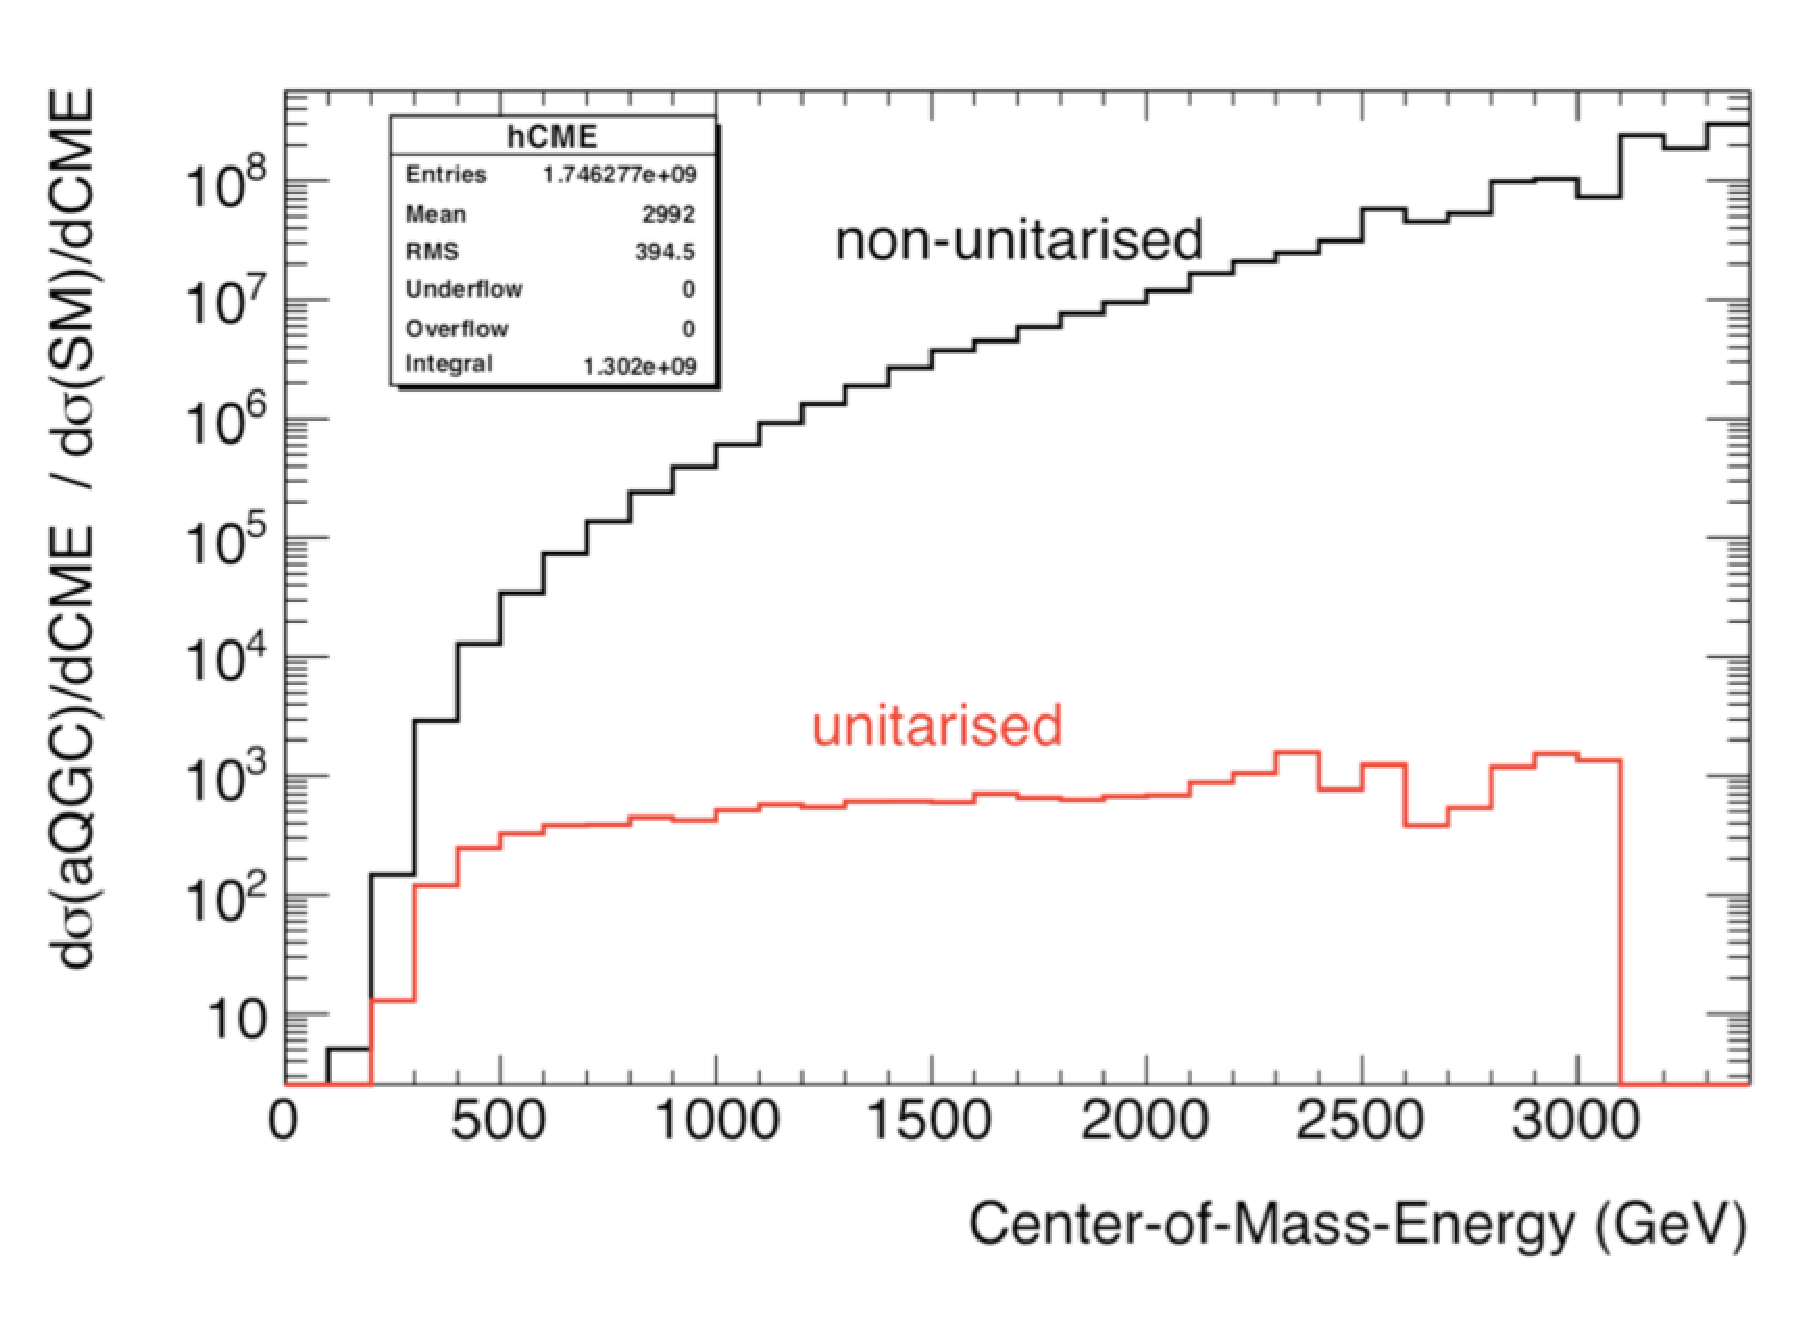
\includegraphics[width=0.8\textwidth]{figures/signal_section/Unitarity_check.eps}  
  \caption{The unitarized and non-unitarized differential cross
    sections as a function of $\sqrt{s}$ for $f_{s0}/\Lambda^4
    = 6\times 10^{-7}~\GeV^{-4}$ divided by the SM values. The
    form factor function with $NF=1$ and $\Lambda_{FF} =$ 180~\GeV is
    used for unitarization.  }
\label{fig:unitaritycheck}
\end{figure}
The simulated aQGC samples were generated with no unitarization schema. For
each of them, we generate two samples of very high statistics with the
same couplings. One of them is unitarized and the other is not. We
derive the weights to weight a non-unitarized sample to a unitarized
sample from the ratio of the distributions of $\sqrt{s}$ of the two
samples of high statistics. The dataset ID, coupling parameters,
non-unitarized cross sections at LO and NLO, $\Lambda_{FF}$ for
unitarization and unitarized cross sections are listed in
Tables~\ref{tab:signalNormaMMP} and~\ref{tab:signalNormaPPM}. The uncertainties on the NLO cross
sections due to scales and PDF are evaluated in the same manner as for
the SM cross sections.
\begin{table}[ht!]
  \centering
  {
\renewcommand{\arraystretch}{1.3}
\begin{tabular}{c|c|c|c|c|c|c}
  \hline
  Sample & $\frac{f_{s0}}{\Lambda^4} $ & $\frac{f_{s1}}{\Lambda^4} $ & $\sigma$@LO  & $\sigma$@NLO & $\Lambda_{FF}$  & unitarized  \\
     & $(10^3~\TeV^{-4})$ & $(10^3~\TeV^{-4})$ & [fb] & [fb] &  (GeV) & $\sigma$ @NLO [fb] \\
\hline \hline
185398 & -10 &	-10 & 33.56 &         44.84$\cdot (100^{+7.2}_{-7.3}\pm3.9  )$\% &           380    &       4.44$\cdot (100^{+2.7}_{-3.3}\pm 2.2)\%$ \\
185399 &  -10 &	-6  &     27.31 &     36.52$\cdot (100^{+6.9}_{-7.9}\pm 3.8 )$\% &      390   &        4.09$\cdot (100^{+2.4}_{-4.1}\pm 2.6 )\%$  \\
185400 &  -10  &  -2  &  24.54  &     32.94$\cdot (100^{+8.1}_{-7.7}\pm3.4  )$\%  &     400      &            3.82$\cdot (100^{+2.9}_{-3.7}\pm 2.2)$\% \\ 
185401 & -10   &  2   &  25.21   &    33.78$\cdot (100^{+8.6}_{-7.1}\pm3.9 )$\%   &    560       &           4.86$\cdot (100^{+3.2}_{-3.4}\pm 2.6)$\%\\ 
185402 & -10   &  6   &  29.25   &    39.16$\cdot (100^{+7.4}_{-9.2}\pm3.9  )$\%   &    430       &           3.90$\cdot (100^{+4.0}_{-2.8}\pm 2.2)$\%\\
185403 & -10   &  10  &  36.73   &    49.06$\cdot (100^{+9.3}_{-7.5}\pm2.5 )$\%   &    440       &           4.16$\cdot (100^{+3.0}_{-3.3}\pm 2.5 )$\% \\
\hline
185404 & -6    &  -10 &  19.96   &    26.80$\cdot (100^{+7.2}_{-7.0}\pm 3.2 )$\%    &   390       &           3.84$\cdot (100^{+3.4}_{-3.0}\pm 2.6)$\% \\ 
185405 & -6    &  -6  &  13.43   &    18.10$\cdot (100^{+7.8}_{-6.3}\pm 3.5 )$\%    &   430       &           3.58$\cdot (100^{+2.4}_{-3.8}\pm 1.9)$\% \\
185406 & -6    &  -2  &  10.34   &    13.88$\cdot (100^{+8.4}_{-5.5}\pm 3.8 )$\%   &    450       &           3.34$\cdot (100^{+2.2}_{-3.8}\pm 2.8)$\% \\
185407 & -6    &  2   &  10.67   &    14.48$\cdot (100^{+6.7}_{-7.7}\pm 2.6 )$\%   &    470       &           3.18$\cdot (100^{+3.6}_{-2.3}\pm 2.3 )$\% \\
185408 & -6    &  6   &  14.38   &    19.19$\cdot (100^{+8.5}_{-8.0}\pm  4.0 )$\%   &    500       &           3.38$\cdot (100^{+3.8}_{-3.2}\pm 2.4)$\%\\
185409 & -6    &  10  &  21.66   &    28.23$\cdot (100^{+8.3}_{-9.8}\pm 6.1 )$\%   &    430       &           3.38$\cdot (100^{+2.8}_{-3.5}\pm 2.0 )$\%\\
\hline
185410 & -2    &  -10 &  13.36   &    18.09$\cdot (100^{+6.0}_{-7.7}\pm  5.0 )$\%   &    410       &           3.53$\cdot (100^{+2.6}_{-3.4}\pm 2.3)$\%\\
185411 & -2    &  -6  &  6.65    &    8.91$\cdot (100^{+5.9}_{-5.6}\pm 3.1  )$\%    &    460       &           3.15$\cdot (100^{+3.0}_{-2.9}\pm 2.4)$\%\\
185412 & -2    &  -2  &  3.24    &    4.49$\cdot (100^{+5.1}_{-3.6}\pm 2.9 )$\%    &    560       &           2.89$\cdot (100^{+2.4}_{-3.1}\pm 2.2)$\%\\
185413 & -2    &  2   &  3.25    &    4.45$\cdot (100^{+4.3}_{-5.1}\pm 2.3 )$\%    &    660       &           2.82$\cdot (100^{+3.7}_{-2.3}\pm 2.4 )$\%\\
185414 & -2    &  6   &  6.64    &    8.62$\cdot (100^{+6.1}_{-6.4}\pm 6.6 )$\%    &    470       &           2.82$\cdot (100^{+2.7}_{-2.9}\pm 2.6)$\%\\
185415 & -2    &  10  &  13.50    &    17.04$\cdot (100^{+4.4}_{-14。1}\pm 11.1 )$\%   &   410       &           3.00$\cdot (100^{+3.5}_{-2.9}\pm 3.1)$\%\\
\hline
185416 & 2     &  -10 &  14.16   &    17.86$\cdot (100^{+9.9}_{-5.2}\pm 6.8 )$\%   &    430       &           3.47$\cdot (100^{+2.8}_{-3.5}\pm 2.3 )$\%\\ 
185417 & 2     &  -6  &  7.03    &    9.20$\cdot (100^{+5.6}_{-8.2}\pm 5.7 )$\%     &   490       &           3.10$\cdot (100^{+2.8}_{-3.3}\pm 2.4)$\%\\
185418 & 2     &  -2  &  3.28    &    4.53$\cdot (100^{+3.1}_{-6.9}\pm 3.6 )$\%    &    730       &           2.89$\cdot (100^{+3.1}_{-3.1}\pm 2.7 )$\%\\
185419 & 2     &  2   &  2.98    &    4.17$\cdot (100^{+3.2}_{-5.6}\pm 3.6 )$\%    &    530       &           2.73$\cdot (100^{+2.4}_{-3.1}\pm 2.3 )$\%\\
185420 & 2     &  6   &  6.08    &    8.29$\cdot (100^{+5.8}_{-6.6}\pm 2.3 )$\%    &    430       &           2.82$\cdot (100^{+2.4}_{-3.6}\pm 2.4 )$\%\\
185421 & 2     &  10  &  12.53   &    16.79$\cdot (100^{+4.3}_{-11.3}\pm 4.1 )$\%   &    390       &           2.97$\cdot (100^{+2.7}_{-2.9}\pm 2.3 )$\%\\
\hline
185422 & 6     &  -10 &  21.95   &    28.97$\cdot (100^{+17.1}_{-3.4}\pm 9.0 )$\%   &    450       &           3.78$\cdot (100^{+2.8}_{-3.3}\pm 2.4 )$\%\\ 
185423 & 6     &  -6  &  14.48   &    19.41$\cdot (100^{+9.2}_{-6.5}\pm 3.7 )$\%   &    560       &           3.76$\cdot (100^{+2.8}_{-3.5}\pm 2.4)$\%\\
185424 & 6     &  -2  &  10.42   &    14.21$\cdot (100^{+9.9}_{-5.3}\pm 3.8 )$\%   &    540       &           3.28$\cdot (100^{+2.1}_{-4.0}\pm 2.5)$\%\\
185425 & 6     &  2   &  9.82    &    13.46$\cdot (100^{+5.4}_{-8.6}\pm 4.8 )$\%   &    470       &           3.08$\cdot (100^{+3.7}_{-2.6}\pm 3.1)$\%\\
185426 & 6     &  6   &  12.63   &    17.11$\cdot (100^{+7.7}_{-6.5}\pm 3.9 )$\%   &    410       &           3.09$\cdot (100^{+3.0}_{-3.1}\pm 2.8 )$\% \\
185427 & 6     &  10  &  18.82   &    25.34$\cdot (100^{+7.1}_{-6.8}\pm 4.4 )$\%   &    370       &           3.17$\cdot (100^{+2.5}_{-3.3}\pm 2.2)$\% \\
\hline
185428 & 10    &  -10 &  36.84   &    49.61$\cdot (100^{+7.5}_{-9.1}\pm  3.8)$\%   &    490       &           4.79$\cdot (100^{+3.6}_{-3.3}\pm 2.5)$\%\\
185429 & 10    &  -6  &  29.18   &    39.54$\cdot (100^{+11.2}_{-6.4}\pm 3.6 )$\%   &    490       &           4.28$\cdot (100^{+3.2}_{-3.4}\pm 2.4 )$\%\\
185430 & 10    &  -2  &  24.82   &    34.04$\cdot (100^{+9.4}_{-6.6}\pm 3.5 )$\%   &    470       &           3.88$\cdot (100^{+3.0}_{-3.6}\pm 2.3)$\%\\
185431 & 10    &  2   &  23.78   &    32.07$\cdot (100^{+8.8}_{-6.6}\pm 3.4 )$\%   &    440       &           3.69$\cdot (100^{+2.3}_{-3.7}\pm 2.1)$\%\\
185432 & 10    &  6   &  26.28   &    35.53$\cdot (100^{+7.9}_{-7.3}\pm 3.4 )$\%   &    390       &           3.54$\cdot (100^{+2.9}_{-3.3}\pm 2.2)$\%\\
185433 &  10   &  10  &  32.15   &    43.31$\cdot (100^{+6.7}_{-8.5}\pm 4.1 )$\%   &    360       &           3.55$\cdot (100^{+2.5}_{-3.6}\pm 2.1)$\%\\
\hline 
\end{tabular}
}
\caption{aQGC samples for $W^-W^+W^-$. The uncertainties for the NLO cross sections are provided : the first uncertainty is for PDF and the second is for scales.}
\label{tab:signalNormaMMP}
\end{table}

\begin{table}[ht!]
  \centering
  {
\renewcommand{\arraystretch}{1.3}
\begin{tabular}{c|c|c|c|c|c|c}
  \hline
  sample ID & $\frac{f_{s0}}{\Lambda^4}  $ & $\frac{f_{s1}}{\Lambda^4} $ & $\sigma$@LO & $\sigma$@\
NLO & $\Lambda_{FF}$ & unitarized $\sigma$ @NLO)\\
     & $(10^3 \TeV^{-4})$ & $(10^3 \TeV^{-4})$ & [fb] & [fb] &  (GeV) & [fb] \\
\hline
185434 & -10   &  -10 &  101.78  &    119.67$\cdot (100^{+7.9}_{-7.9}\pm 3.6  )$\%  &        380     &           8.75$\cdot (100^{+2.7}_{-3.5}\pm 2.6 )$\% \\
185435 & -10   &  -6  &  83.20    &    97.87$\cdot (100^{+7.0}_{-9.0}\pm 3.7 )$\%   &       390     &           8.04$\cdot (100^{+2.8}_{-3.3}\pm  2.1)$\% \\
185436 &  -10  &  -2  &  75.86   &    88.44$(100^{+7.6}_{-9.0}\pm  3.8)$\%   &        400     &           7.51$\cdot (100^{+2.8}_{-3.0}\pm 2.1)$\% \\
185437 &  -10  &  2   &  79.12   &    91.60$(100^{+6.9}_{-10.7}\pm 5.0  )$\%    &       560     &           9.98$\cdot (100^{+3.2}_{-3.4}\pm 2.4 )$\% \\
185438 &  -10  &  6   &  93.02   &    107.73$(100^{+9.7}_{-8.1}\pm 2.9  )$\%  &        430     &           7.68$\cdot (100^{+2.3}_{-3.8}\pm 2.0)$\% \\
185439 &  -10  &  10  &  118.34  &    135.00$(100^{+9.5}_{-8.7}\pm 4.3 )$\%     &     440     &           8.40$\cdot (100^{+2.3}_{-4.1}\pm 2.2)$\% \\
\hline
185440 & -6    &  -10 &  58.84   &    70.39$(100^{+6.5}_{-8.2}\pm 3.4 )$\%   &        390     &           7.44$\cdot (100^{+2.1}_{-3.9}\pm 2.4 )$\% \\
185441 &  -6   &  -6  &  39.23   &    46.96$(100^{+7.1}_{-7.7}\pm 3.5 )$\%   &        430     &           6.97$\cdot (100^{+3.5}_{-2.7}\pm 3.1 )$\% \\
185442 & -6    &  -2  &  30.28   &    36.45$(100^{+7.0}_{-8.1}\pm 3.2 )$\%   &        450     &           6.35$\cdot (100^{+2.0}_{-4.1}\pm 2.3 )$\% \\
185443 & -6    &  2   &  32.17   &    38.04$(100^{+8.8}_{-7.1}\pm  2.9 )$\%   &        470     &           6.20$\cdot (100^{+2.5}_{-3.8}\pm 2.3)$\% \\
185444 & -6    &  6   &  44.86   &    52.28$(100^{+6.5}_{-9.7}\pm 4.7 )$\%   &        500     &           6.65$\cdot (100^{+2.7}_{-3.5}\pm 2.4 )$\% \\
185445 &  -6   &  10  &  68.00      &    75.46$(100^{+3.4}_{-17.5}\pm 4.9 )$\%   &     430     &           6.65$\cdot (100^{+2.8}_{-3.2}\pm 2.4 )$\%\\
\hline
185446 & -2    &  -10 &  39.50    &    46.00$(100^{+5.4}_{-10.0}\pm 5.1 )$\%      &    410     &           6.75$\cdot (100^{+1.8}_{-4.2}\pm 2.5)$\% \\
185447 & -2    &  -6  &  18.10    &    21.40$(100^{+7.8}_{-5.3}\pm 4.9 )$\%    &      460     &           6.11$\cdot (100^{+3.9}_{-2.5}\pm 3.1 )$\% \\
185448 & -2    &  -2  &  7.71    &    9.95$(100^{+3.3}_{-6.5}\pm 3.8 )$\%    &        560     &           5.48$\cdot (100^{+5.2}_{-1.4}\pm 3.2 )$\% \\
185449 & -2    &  2   &  8.12    &    10.08$(100^{+9.6}_{-3.4}\pm 4.8 )$\%   &        660     &           5.31$\cdot (100^{+2.9}_{-2.9}\pm  2.7)$\% \\
185450 & -2    &  6   &  19.23   &    21.76$(100^{+4.5}_{-14.9}\pm 6.1 )$\%   &        470     &           5.41$\cdot (100^{+2.9}_{-3.0}\pm 2.6 )$\% \\
185451 & -2    &  10  &  41.19   &    44.66$(100^{+7.3}_{-11.6}\pm  10.6)$\%   &        410     &           5.76$\cdot (100^{+3.4}_{-2.6}\pm 2.6 )$\% \\
\hline
185452 & 2     &  -10 &  42.97   &    48.64$(100^{+3.3}_{-15.5}\pm  4.6)$\%   &        430     &           6.69$\cdot (100^{+2.6}_{-3.3}\pm 2.5  )$\% \\
185453 & 2     &  -6  &  19.86   &    22.64$(100^{+4.4}_{-10.8}\pm 4.6 )$\%   &        490     &           5.99$\cdot (100^{+2.5}_{-3.2}\pm 2.6 )$\% \\ 
185454 & 2     &  -2  &  8.18    &    10.07$(100^{+6.4}_{-5.0}\pm  3.9)$\%   &        730     &           5.52$\cdot (100^{+2.3}_{-3.2}\pm 3.1)$\% \\
185455 & 2     &  2   &  7.12    &    9.17$(100^{+6.2}_{-3.7}\pm 3.1 )$\%    &        530     &           5.03$\cdot (100^{+2.4}_{-3.3}\pm 2.2)$\% \\
185456 & 2     &  6   &  16.99   &    20.36$(100^{+5.3}_{-8.2}\pm 3.9 )$\%   &        430     &           5.26$\cdot (100^{+3.5}_{-2.3}\pm 3.0)$\% \\
185457 & 2     &  10  &  37.28   &    44.77$(100^{+12.0}_{-3.8}\pm 7.6  )$\%   &        390     &           5.69$\cdot (100^{+2.0}_{-3.6}\pm 2.2 )$\% \\ 
\hline
185458 &  6    &  -10 &  69.13   &    76.41$(100^{+6.1}_{-9.7}\pm 11.4 )$\%   &        450     &           7.41$\cdot (100^{+3.1}_{-3.1}\pm 3.0 )$\% \\
185459 & 6     &  -6  &  45.00      &    51.40$(100^{+6.5}_{-10.0}\pm 5.4  )$\%    &     560     &           7.49$\cdot (100^{+2.6}_{-4.0}\pm 2.7)$\% \\
185460 & 6     &  -2  &  31.70    &    37.58$(100^{+7.7}_{-9.2}\pm 5.4 )$\%   &       540     &           6.40$\cdot (100^{+2.6}_{-3.5}\pm 2.4)$\% \\
185461 & 6     &  2   &  29.15   &    35.00$(100^{+7.0}_{-8.2}\pm 3.1 )$\%      &     470     &           5.94$\cdot (100^{+2.8}_{-3.3}\pm 2.3)$\% \\
185462 & 6     &  6   &  37.40    &    44.85$(100^{+5.5}_{-9.9}\pm 4.3 )$\%   &       410     &           5.84$\cdot (100^{+2.3}_{-3.6}\pm 2.2)$\% \\
185463 &  6    &  10  &  56.49   &    67.15$(100^{+7.5}_{-8.0}\pm 3.8)$\%   &        370     &           6.13$\cdot (100^{+2.3}_{-3.0}\pm 2.4)$\% \\
\hline
185464 & 10    &  -10 &  118.00     &    137.09$(100^{+9.2}_{-9.2}\pm 4.2  )$\%  &     490     &           9.85$\cdot (100^{+2.6}_{-4.3}\pm 2.4)$\% \\
185465 & 10    &  -6  &  93.09   &    108.25$(100^{+8.2}_{-9.9}\pm 4.0)$\%  &        490     &           8.64$\cdot (100^{+2.9}_{-3.7}\pm 2.7)$\% \\
185466 & 10    &  -2  &  77.80    &    91.46$(100^{+8.6}_{-8.7}\pm 3.6 )$\%   &       470     &           7.81$\cdot (100^{+1.9}_{-4.7}\pm 2.7 )$\% \\
185467 & 10    &  2   &  74.29   &    87.16$(100^{+8.0}_{-8.9}\pm  4.3)$\%   &        440     &           7.30$\cdot (100^{+3.3}_{-2.9}\pm 3.2)$\% \\
185468 & 10    &  6   &  81.13   &    95.43$(100^{+7.9}_{-8.3}\pm 4.1)$\%   &        390     &           6.90$\cdot (100^{+2.5}_{-4.1}\pm 2.8)$\% \\
185469 & 10    &  10 &   98.57   &    117.14$(100^{+7.3}_{-9.1}\pm 4.0 )$\%  &        360     &           7.01$\cdot (100^{+3.1}_{-2.8}\pm 2.6)$\% \\
\hline
\end{tabular}
}
\caption{aQGC samples for $W^+W^+W^-$. The uncertainties for the NLO cross sections are provided : the first uncertainty is for PDF and the second is for scales.}
\label{tab:signalNormaPPM}
\end{table}





















